\chapter{روش‌های مبتنی بر شبکه‌ی عصبی}
\todo{مقدمه؟}



%  یکی از مشکلات مدل ترنسفومر در خلاصه‌سازی متون طولانی حافظه‌ی درجه دوم پیچیدگی‌های محاسباتی و تعداد زیاد عملیات می‌باشد. برای حل این مشکلات کار‌های مختلفی انجام شده است. به عنوان مثال شبکه‌ی رفورماتور2 [24] از درهم‌سازی حساس به محل3 برای محاسبه وزن‌های توجه استفاده می‌کند و پیچیدگی حافظه را به کاهش می‌دهد. همچنین شبکه‌ی ترانسفورمر پراکنده [18] با معرفی فاکتورسازی‌ ماتریس پراکنده‌ی توجه، زمان و حافظه مورد نیاز را به کاهش می‌دهد. مدل بیگ برد4 [17] با استفاده از مکانیزم توجه پراکنده5 که وابستگی را به خطی کاهش ‌می‌دهد و عملکرد ترنسفورمر را در مواجه با توالی6 طولانی بهبود می‌بخشد.  در سال‌های اخیر مدل‌های مختلفی برای بهبود کیفیت خروجی مدل خلاصه‌سازی خودکار اسناد بلند ارائه شده است. به عنوان مثال ژیائو و کارنی7 [16] با تمرکز برکاهش تکرار و افزونگی در خلاصه سازی اسناد طولانی مدلی طراحی کرده‌اند که کدگشایی آن براساس مکانیزم توجه آگاه از افزونگی می‌باشد. علاوه بر این تابع هزینه‌ای8 طراحی کرده‌اند که برای تعادل بین اهمیت و افزونگی مناسب باشد. این روش باعث انتخاب جملات مهم و غیر زائد می‌شود. پایلو9 و همکاران [4] که برای بهبود خلاصه انتزاعی نهایی متون طولانی از رویکرد ترکیبی استخراجی-انتزاعی با استفاده از مدل زبانی از پیش آموزش دیده GPT$_2 [12]$ استفاده می‌کنند. در این مدل مرحله استخراج ساده قبل از تولید خلاصه انجام می‌شود، سپس برای شرطی کردن مدل زبانی ترنسفورمر بر روی اطلاعات مربوط قبل از تولید خلاصه استفاده می‌شود. این رویکرد در مقایسه با کارهای قبلی که از مکانیزم کپی استفاده می‌کنند، خلاصه‌های انتزاعی بیشتری تولید می‌کند.  پانگ10 و همکاران [15] یک ساختار سلسله مراتبی برای اسناد طولانی فرض کرده‌اند. در این ساختار سطح بالا بر وابستگی دوربرد تمرکز می‌کند و سطح پایین جزئیات را حفظ می‌کند. این چارچوب استنتاج از پایین به بالا را با استنتاج از بالا به پایین برای بهبود استنتاج نمایش توکن هم‌افزایی می‌کند. در حال حاضر این روش بهترین عملکرد را در خلاصه‌سازی متون طولانی دارد. همچنین این روش خلاصه‌سازی در اسناد کوتاه حافظه بهینه‌تر و کارایی محاسباتی بالاتر دارد.


\section{روش‌های مبتنی بر مدل کدگذار-کدگشا}
قبل از ظهور ترنسفورمرها ، مدل‌های شبکه عصبی عمیق دنباله به دنباله بهترین مدل‌ها برای وظایف تولید متن از جمله ترجمه‌ی ماشینی و خلاصه‌سازی متن بوده‌اند. این مدل‌ها ورودی را از یک فرم به فرم دیگر نگاشت می‌کنند تا نتایج مورد نظر را تولید کنند. معماری کدگذار-کدگشا رویکرد اصلی برای مدل‌سازی مدل‌های دنباله به دنباله است. شکل \ref{fig:encoder_decoder} معماری پایه‌‌ی مدل  کدگذار-کدگشا را شرح می‌دهد.
شبکه‌های بازگشتی
\LTRfootnote{recurrent neural network (RNN)}
\cite{elman1990finding}
و حافظه‌های کوتاه مدت طولانی
\cite{hochreiter1997long}
برای توالی طراحی شده‌اند و مناسب‌ترین معماری‌های یادگیری عمیق برای کدگذاری و پردازش داده‌های دنباله‌ای مانند متن هستند. اما این شبکه‌ها در مدیریت حافظه‌ی بلند مدت طولانی
\LTRfootnote{long short-term memory networks(LSTM)}
مشکل دارند.
\begin{figure}[!h]
	\begin{center}
		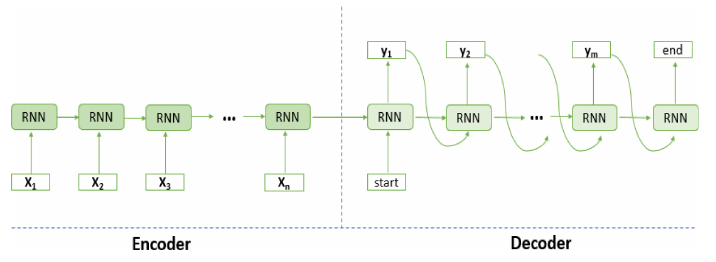
\includegraphics[height=4cm]{encoder_decoder.png}
	\end{center}
	\caption{معماری پایه‌‌ی مدل  کدگذار-کدگشا\cite{ALOMARI2022101276}}
	\label{fig:encoder_decoder}
	\medskip
	\small
\end{figure}

یکی از مدل‌های کدگذار-کدگشای ارایه شده مدل سلسله مراتبی متغیر برای خلاصه‌سازی متقابل زبانی
\LTRfootnote{cross-lingual}
می باشد.  مدل پیشنهادی شامل دو متغیر نهفته محلی، یکی برای ترجمه و دیگری برای خلاصه سازی، و یک متغیر نهفته جهانی برای خلاصه سازی بین زبانی است. متغیرهای پنهان محلی به ترتیب برای بازسازی ترجمه و خلاصه زبان مبدأ محدود می شوند. سپس از متغیر پنهان سراسری برای تولید خلاصه بین زبانی استفاده می شود. قسمت کد گذار دو بخش دارد که هر بخش وظیفه‌ی تولید یکی از متغیرهای پنهان محلی را دارد.
بخش کدگشا با استفاده از نمایش‌های نهفته‌ی محلی خلاصه‌ی نهایی را تولید می‌کند.
ساختار سلسله مراتبی مدل به آن اجازه می دهد تا رابطه سلسله مراتبی بین ترجمه، خلاصه سازی و خلاصه سازی بین زبانی را بیاموزد.






\begin{figure}[!h]
	\begin{center}
		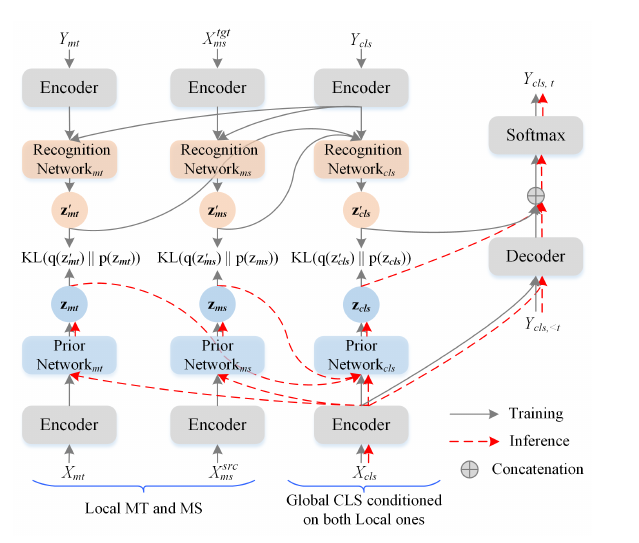
\includegraphics[height=9cm]{Variational Hierarchical Model.png}
	\end{center}
	\caption{معماری پایه‌‌ی مدل سلسله مراتبی متغیر برای خلاصه‌سازی متقابل زبانی\cite{variational}}
	\label{fig:vahie_model}
	\medskip
	\small{
		متغیرهای محلی $ z_mt $ و $ z_ms $ به ترتیب برای ترجمه و خلاصه سازی طراحی شده اند. سپس $ z_cls $ جهانی برای خلاصه سازی بین زبانی است، خطوط خاکستری ن نشان‌دهنده فرآیند آموزشی است که مسئول تولید
		($ z' _{mt} $، $ z'_{ms} $، $ z'_{cls} $)
		از توزیع پسین متناظر پیش‌بینی‌شده توسط شبکه‌های شناسایی است که یادگیری شبکه‌های قبلی را هدایت می‌کند.خطوط قرمز چین نشان دهنده فرآیند استنتاج برای تولید نمایش‌‌های نهفته
		($ z _{mt} $، $ z_{ms} $، $ z_{cls} $)
		از توزیع های قبلی مربوطه پیش بینی شده توسط شبکه های قبلی است  }
\end{figure}



%\subsection{روش‌های ارايه شده برای متون کوتاه }


%\subsection{روش‌های ارايه شده برای متون طولانی }


\section{روش ‌های مبتنی بر مدل ترنسفورمر ها}
با ظهور ترنسفورمرها \cite{vaswani2017attention}، بهبودهای قابل توجهی در کیفیت نتایج خلاصه‌سازی خودکار به وجود آمد. ترنسفومرها با استفاده از مکانیزم توجه به خود‏
\LTRfootnote{Self-attention}
شباهت بین ورودی‌ها را بدون توجه به موقعیت موازی آن‌ها با حضور مستقل هر توکن در توالی ورودی مدل می‌کنند و به طور مؤثر مشکلات شبکه‌های بازگشتی را حل می‌کنند. یکی از جهت‌گیری‌های رایج پژوهشی، اصلاح یا تطبیق ترنسفورمرها و مدل‌های زبانی از پیش آموزش دیده با وظایف مختلف مانند خلاصه‌سازی است. مدل‌های مبتنی بر مدل‌های زبانی از پیش آموزش دیده که با هدف خلاصه‌سازی انتزاعی طراحی شده‌اند از ویژگی‌های معنایی و متنی غنی بازنمایی‌های زبان برای بهبود کیفیت و دقت خلاصه‌‌ها استفاده می‌کنند.
\\
به عنوان مثال مدل پگاسوس
\LTRfootnote{PEGASUS}
\cite{zhang2020pegasus}
یک مدل دنباله به دنباله کدگذار کدگشا مبتنی بر ترنسفورمر است که بر روی مجموعه‌های متنی بدون نظارت با هدف تولید جملات شکاف
\LTRfootnote{‫‪gap‬‬ ‫‪sentences‬‬ ‫‪generation‬‬}
از قبل آموزش داده شده است. این مدل عملکرد مناسبی در خلاصه‌سازی متون کوتاه دارد. در حال حاضر بهترین مدل خلاصه‌سازی متون کوتاه مبتنی بر مدل پگاسوس است
\cite{sherborne2023meta}.

\section{روش های مبتنی بر مدل‌های از پیش آموزش دیده}




\section{ایده های  ارایه شده بهبود خلاصه سازی متون طولانی }

\todo{کوتاه بلند از مقاله بنویس}

جیدیوتیس و همکاران  شیوه‌ی تقسیم و غلبه ( دنسر) 
\LTRfootnote{Divide-ANd-ConquER (DANCER)}
را  برای بهبود خلاصه سازی اسناد طولانی پیشنهاد کرده اند.این روش به طور خودکار خلاصه یک سند را به چند بخش‌ تقسیم می‌کند و هر یک از این بخش‌ها را به بخش مناسب سند جفت می‌کند تا خلاصه‌های هدف متمایز ایجاد کند. شیوه‌ی معرفی شده در نظر می‌گیرد که متون طولانی به صورت بخش‌های گسسته ساختاربندی شده‌اند. 

برای مطابقت هر قسمت از خلاصه با بخشی از سند در دنسر از معیار روژ 
\LTRfootnote{ROUGE}
استفاده  ‌می‌شود. در این روش معیار روژ-ال بین هر یک از جملات خلاصه و تمام جملات سند محاسبه می‌شود و هر جمله ی خلاصه هدف به بخش حاوی جمله با بیشترین روژ- ال نسبت داده می‌شود. 
سپس تمام جملات خلاصه‌ی هدف مربوط به هر بخش را به هم الحاق می کنیم تا خلاصه‌ی هدف برای هر بخش ایجاد شود. در طول آموزش هر بخش از سند به همراه جمله‌ی خلاصه‌ی مربوط به آن به عنوان متن ورودی و خلاصه‌ی هدف استفاده می‌شود. 
مزایای این روش آموزش:
\begin{enumerate}
	\item {
		 تقسیم مساله به چند زیر مساله باعث کاهش پیچیدگی و ساده‌سازی مساله می‌شود.
	}
	\item {
		انتخاب خلاصه‌های هدف برای هر بخش بر اساس امتیازات روژ-ال هر جمله باعث تطابق بهتر و متمرکزتر بین دنباله‌های منبع و هدف ایجاد می‌شود.
	}
	\item {
تقسیم هر سند آموزشی به چند جفت ورودی-هدف، نمونه های آموزشی بسیار بیشتری ایجاد می کند. این کار برای مدل‌های خلاصه‌سازی عصبی مفید است. 	
}
	\item {
	این روش می‌تواند از مدل‌های خلاصه‌سازی مختلف از جمله شبکه‌ی عصبی بازگشتی و ترنسفورمرها استفاده کند.
}
\end{enumerate}


هنگام کار با اسناد ساختاریافته طولانی، معمولاً همه بخش‌های سند کلیدی برای سند نیستند. اگر یک مقاله آکادمیک را به عنوان مثال در نظر بگیریم، بخش هایی مانند مرور ادبیات یا پیشینه در تلاش برای خلاصه کردن نکات اصلی مقاله ضروری نیستند و باعث افزودن نویز می‌شوند. بنابراین از بخش مرور ادبیات صرف نظر می‌شود و تمرکز سیستم خلاصه‌سازی فقط  روی بخش‌های مقدمه، روش‌ها، نتایج و نتیجه‌گیری می‌باشد.
\todo{میتونه حذف بشه }

این مدل قابل ترکیب با پگاسوس یا مدل مولد نقطه‌ای 
\LTRfootnote{Pointer-Generator model}
می‌باشد.
بخش کدگشا مدل مولد نقطه‌ای با ایجاد جملات تکراری مقابله ‌می‌کند.
هرچند ممکن است به خاطر تکرار اطلاعات در بخش های مختلف بازهم خلاصه‌ی تکراری ایجاد شود.






